%-------------------------------------------------------------------------------
% BOARD ENCODING
%-------------------------------------------------------------------------------
\subsection{Board encoding}

\begin{frame}{``Cogito" system overview}{Board encoding}

\begin{block}{First-order logic}
  \begin{itemize}
    \item translation- and rotation-invariant,
    \item pattern-matching using homomorphisms.
  \end{itemize}
\end{block}
\pause
%\begin{exampleblock}
\begin{figure}[ht]
  \begin{minipage}[t]{0.4\linewidth}
    \vspace{0pt}
    \centering
    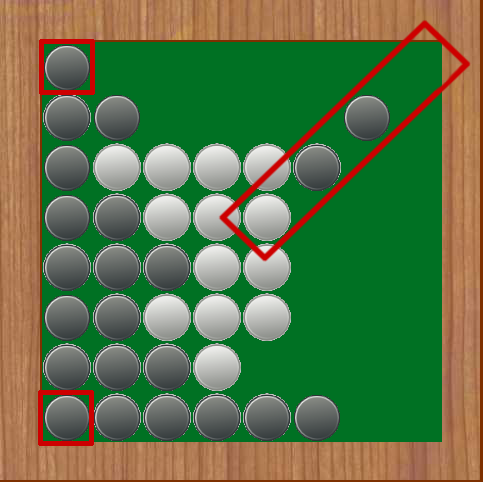
\includegraphics[width=0.8\textwidth]{img/cogito/raisonneur_choix_2}	
  \end{minipage}
  \hfill
  \begin{minipage}[t]{0.55\textwidth}
    \vspace{0pt}
    \begin{itemize}
	\item $isCorner(x) \wedge isMine(x)$
	\item $isMine(w) \wedge isOpp(x) \wedge isOpp(y) 
		  \wedge aligned(w,x,y) \wedge isEmpty(z) 
		  \wedge aligned (x,y,z)$
    \end{itemize}
  \end{minipage}
\end{figure}
%\end{exampleblock}

\end{frame}

%-------------------------------------------------------------------------------
% MEMORY STRUCTURE
%-------------------------------------------------------------------------------
\subsection{Memory structure}
\begin{frame}{``Cogito" system overview}{Memory structure}

\begin{block}{Remember}
Objects are board-states, attributes are local configurations.
\end{block}

\begin{figure}[ht]
  \begin{minipage}[t]{0.45\linewidth}
    \vspace{0pt}
    \centering
    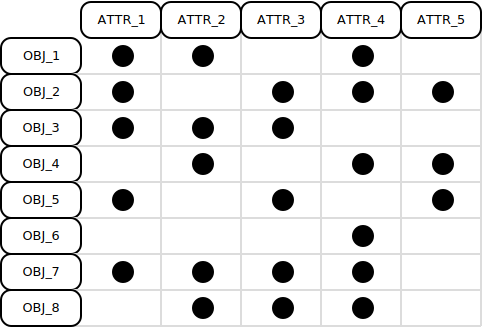
\includegraphics[width=\textwidth]{img/cogito/context_matrix}
    \\ Matrix representation
  \end{minipage}
  \hfill
  \begin{minipage}[t]{0.45\textwidth}
    \vspace{0pt}
    \centering
    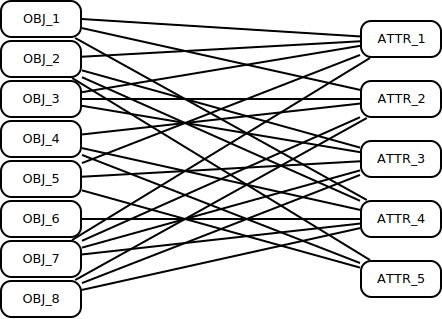
\includegraphics[width=\textwidth]{img/cogito/context_graph}
    \\ Graph representation
  \end{minipage}
\end{figure}

\end{frame}




%-------------------------------------------------------------------------------
% EVALUATING CONFIGURATIONS
%-------------------------------------------------------------------------------
\subsection{Evaluating configurations}
\begin{frame}{``Cogito" system overview}{Evaluating configurations}

When the game ends the final configuration is given a value based on whether the 
agent has won or last. This value and is propagated backwards through previous
board states with linear attenuation. The value of a state board the value 
of its configurations.

\end{frame}

%-------------------------------------------------------------------------------
% GENERATING NEW CONFIGURATIONS
%-------------------------------------------------------------------------------
\subsection{Generating new configurations}
\begin{frame}{``Cogito" system overview}{Generating new configurations}

New relevant configurations are deduced by attempting to locally extend an 
existing configuration shared by two or more winning or losing board states.

\end{frame}

%-------------------------------------------------------------------------------
% PUTTING IT ALL TOGETHER
%-------------------------------------------------------------------------------
\subsection{Putting it all together}
\begin{frame}{``Cogito" system overview}{Putting it all together}

The system receives a set of possible moves to choose from. By evaluating each 
resulting board state based on prior experience it is able to choose the one 
which seems most beneficial.

Nota Bene: there is no look-ahead, but as we are essentially engineering a 
dynamic heuristic the system could be easily combined with a limited-depth 
Minimax implementation.

\end{frame}